\section{Tuesday, February 7th: Conceptual Models (continued)}
We start at the \textbf{Design Model} and then go to the \textbf{System Image} which then iterates back and forth between itself and the \textbf{User's Model}.

It is important to realize that the User's Model is \textit{different} than the System Image -- the User cannot see your source code!

\subsection{Make Controls Visible}
Hidden side buttons or controls in hard-to-reach places will make it so that users don't know or won't use features.

\subsubsection{Don't overload the User}
``Too Much Visibility?'' is a thing and will make it had for the user to find the 1 button they want to press amongst the 200 available choices. Note that we will later formalize this with a function that measures visual search cost (More buttons $\implies$ longer processing time to find a button).

\subsubsection{Make Controls Clear}
A lot of seat controls have clear mappings from what you want to have happen to the action needed to make that a reality.

\subsubsection{Case Study: Stovetop Controls}
Which knob controls which burner on a stove is a classic UI question.

Contrary to common opinion, you do not actually need labels to make this unambiguously clear. All you need is to arrange the stoves in a non-linear manner and have the knobs be perturbed in the same manner:
\begin{figure}[H]
    \centering
    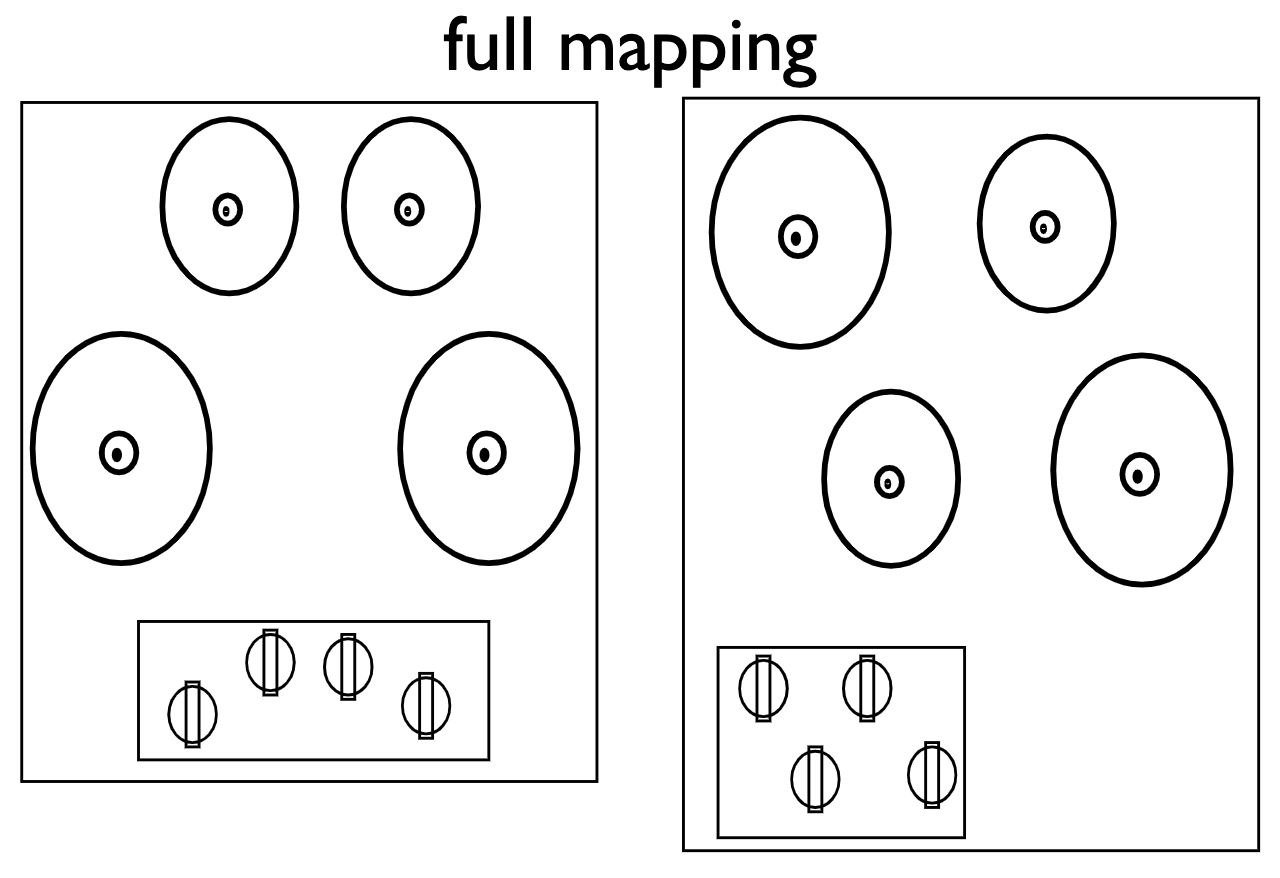
\includegraphics[scale=0.2]{lectures/wk4/img/stove.png}
    \caption{This is unambiguously clear since the knobs are not packed in a horizontal line}
    \label{fig:stove}
\end{figure}

\subsubsection{Use Transfer Learning}
Knowledge from other domains can help users understand how new technologies can work. Laptops have keyboards in a layout that mimics those of typewriters to help people transition to newer technology.

\subsubsection{Provide Feedback}
\begin{shaded}
Q: Have you ever pressed a button more than once? If so, why?
\end{shaded}
The answer is likely that you did not recieve timely feedback that your input was registered (perhaps you did not press hard enough?).

Making sure you have low-latency is key for good UX.

\subsection{Action Cycle}
\begin{figure}[H]
    \centering
    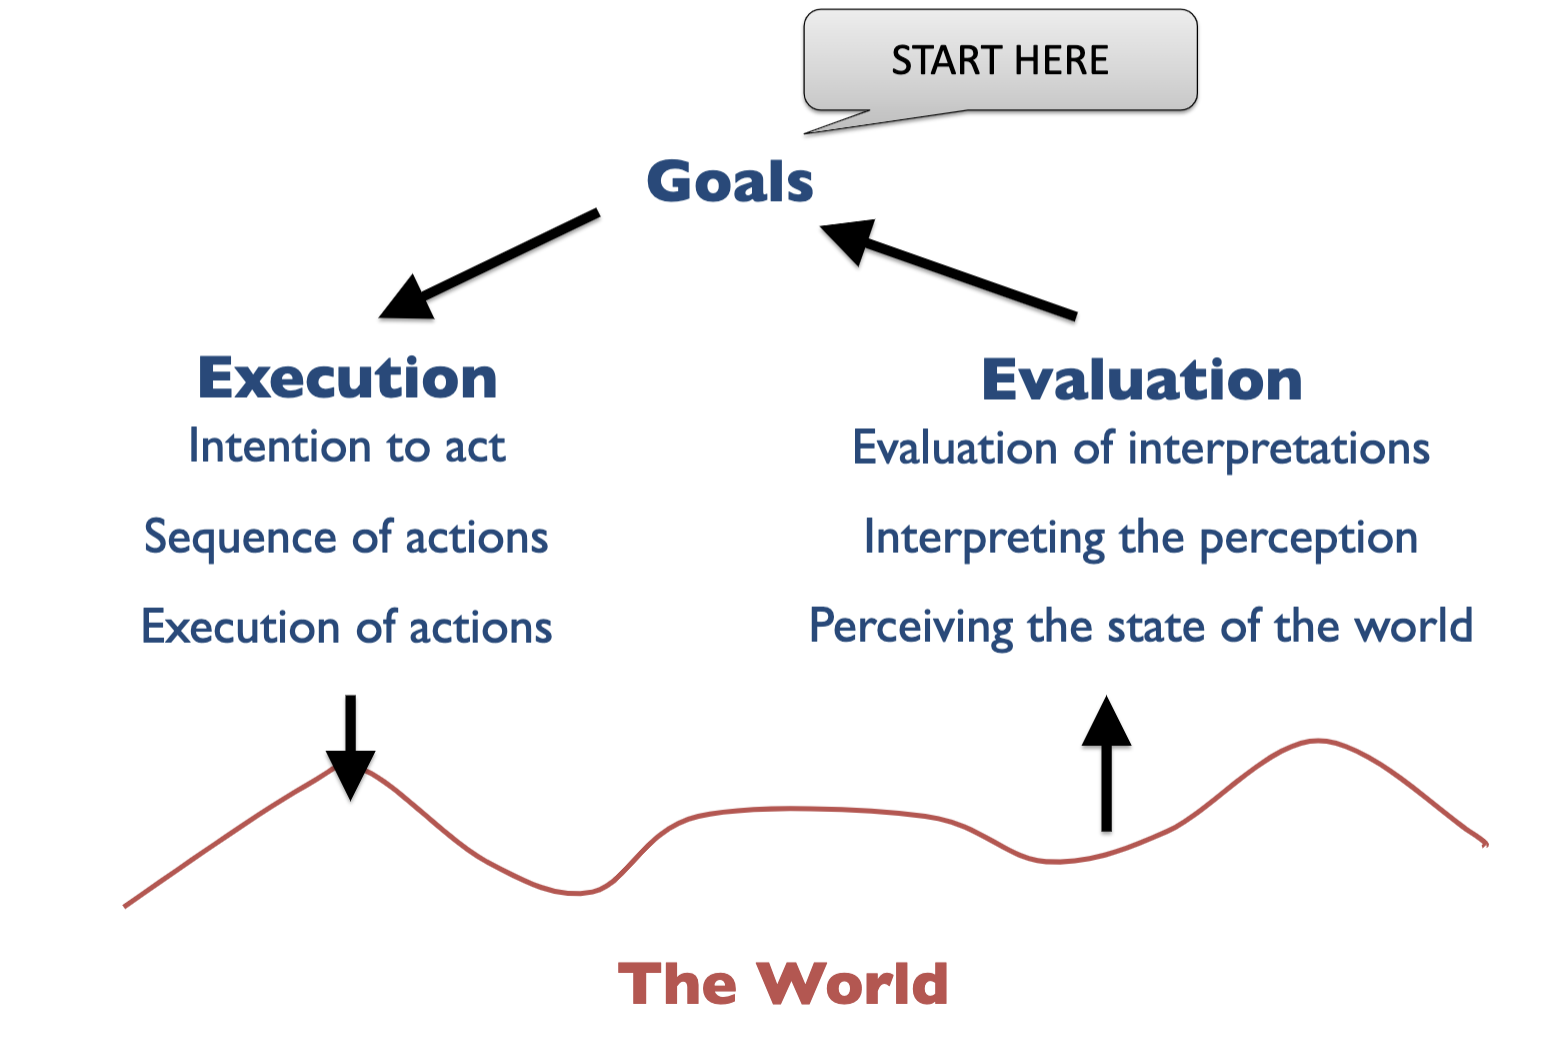
\includegraphics[scale=0.2]{lectures/wk4/img/action_cycle.png}
    \caption{This is a diagram of the Action Cycle}
    \label{fig:action_cycle}
\end{figure}

\subsubsection{Gulf of Evaluation}
Let us say that you are a Data Scientist who is trying to figure out some correlations.

If I can you some pairs of $(x, y)$ in an unsorted order this would be a very non-trivial task. Your first thought may be to re-order the data.

However what if I give you the data as a scatterplot. Then it may be a bit easier to immediately answer as we can use our perceptual systems.

\subsubsection{Gulf of Execution}
What if I ask you to draw some complicated shapes with a turtle drawing program?

This is non-trivial as you need to calculate some trigonometry. However if I gave you some `draw some shape' command then it would be much easier to execute this task. Note that the Execution is abstracted -- when coding we generally don't think about what is being put into each register in the generated Assembly code.

\begin{shaded}
    Gulf of Evaluation goes from  \textit{Mental Model} to the \textit{Real World}.
\end{shaded}

\subsection{Interface Languages}
\begin{shaded}
    An \textbf{interface language} is the set of actions a user can take in an 
interface. These actions have abstract \textit{meaning} and a concrete \textit{physical 
form}.  You can define its input language (provided by user to app) and 
its output language (provided by app to user)
\end{shaded}

\subsubsection{Semantic \& Articulatory Distance}
\begin{shaded}
\textbf{Semantic} distance reflects the relationship between the \textit{user’s 
intentions} and the \textit{meaning of expressions} in the interface languages.
% This is the distance between what you want 

\textbf{Articulatory} distance reflects the relationship between the \textit{physical 
form} of an expression in the interaction language and its \textit{meaning}.
% This is like what you have to do for 
\end{shaded}

\subsubsection{Case Study: Adding Autocomplete}
Q: If you added autocomplete to your app, would you be adding Semantic or Articulatory Distance? Would this narrow the gulf of execution or evaluation?

A: This is a trick question -- it can be both the gulf of execution (you need to type less keystrokes -- lower articulatory distance as you need to do less physical actions) or narrow the gulf of evaluation (as you get to see similar searches -- if you don't know how to spell something, your intentions can still be understood and met).

\subsubsection{Spell and Grammar Suggestions}
Gulf of evaluation (looking at what the UI shows you and interpreting ``did this meet my goal or not'') and semantic distances are both lowered since our intention gets matched up to the real world.

\subsection{Direct Manipulation}
An interface that behaves as though the interaction was with a real-world object rather than with an abstract system

Central ideas
\begin{enumerate}
    \item Visibility of the objects of interest
        \begin{itemize}
            \item If you open a phone, your apps are instantly viewable
        \end{itemize}
    \item Rapid, reversible, incremental actions
        \begin{itemize}
            \item You can undo actions
        \end{itemize}
    \item Manipulation by pointing and moving
        \begin{itemize}
            \item You can scroll between apps with ease
        \end{itemize}
    \item Immediate and continuous display of results
        \begin{itemize}
            \item There are no hidden states, or compiling, WYSIWYG (what you see is what you get)
        \end{itemize}
\end{enumerate}
GUIs were formed by HCI experts so that people in this room (i.e. non-CS majors) can work with technology.

\begin{important}
Note that if you have used something like \LaTeX\ then that is an example of something that is not direct manipulation.
\end{important}

Voice control (like Siri) narrows the Gulf of Execution.

\subsection{Metaphor}
\begin{shaded}
    \textbf{Metaphor} -- The transference of the relation between one set of objects to another set for the purpose of brief explanation
\end{shaded}

This can be useful to help clue users in what the functionality of an interface is and how it might be used.

Not all signifiers are metaphors -- metaphors are a type of signifier -- all metaphors lend themselves to affordances.

\subsection{Modes}
This can be useful in applications like Photoshop or Illustrator.

However this can be bad for the User as they need to remember what mode they are in. The SFO airplane crash we talked about in lecture 1 was due to the Pilot thinking they were on autopilot when they were not.

\subsubsection{Fixing the Problems with Modes}
\begin{itemize}
    \item Simply do not use modes
    \item Make it very explicitly clear which mode you are in
\end{itemize}

The easiest way to go about the second option is to make a redundant UI for the additional modes.

\subsubsection{Quasimodes}
You have to consciously and continuously take some action to stay in the mode.

The best example of this is the \texttt{Shift} key, where if you let go then you exit the mode. This makes sense as you more often than not want to type in lowercase.

This is different from the \texttt{Caps Lock} key which completely switches your mode (which can lead to the accident where you write a bunch of text in all caps, essentially unintentionally `yelling' at someone).
